\chapter{让结构直接解释重叠像素}
\section{用一个共同结构连接多个区域}
逐个重叠点去孪晶，要求每一组像素独立确定所有分量。这个要求有时过强，因为各个反射来自同一个原子结构。可以先保留第三章的观测似然，再把结构预测代入：
\begin{equation}\label{eq:joint-residual}
 r_g(\theta,\alpha)=R_g\diag(c_g\alpha_{d_g})\,k|F_{h_g}(\theta)|^2-z_g.
\end{equation}
联合目标是
\begin{equation}
 Q(\theta,\alpha)=\sum_{g\in\mathcal W}\bigl[\|r_g\|^2+c_g^{\rm residual}\bigr]
                  +Q_{\rm restraints}(\theta).
\end{equation}
这里的 $c_g$ 是各分量校正系数向量，$c_g^{\rm residual}$ 是压缩残差常数，两者不要混淆。每个分量有独立的 Miller 指数和所属晶畴编号。多个晶畴共享一个结构的前提是它们属于同一相，接口要求显式声明这一点。

对于背景已按线性高斯模型消元的像素，这个目标与在原始像素上逐次重估背景的目标相同。精修没有把相关估计变成独立行，也没有先求一张唯一的去孪晶强度表。

\section{解析导数如何穿过观测算子}
令 $v_g(\theta)=k|F_{h_g}(\theta)|^2$。结构参数和晶畴比例的 Jacobian 分别为
\begin{align}
 \partial_\theta r_g&=R_g\diag(c_g\alpha_{d_g})\,\partial_\theta v_g,\\
 \partial_u r_g&=R_g\diag(c_gv_g)\,\partial_u\alpha_{d_g}.
\end{align}
前一章的衍射导数可以直接复用；第二式使用 softmax 的导数。整个结构精修看到的是小型 $R_g$，不用重复加载大量高斯像素。若轮廓、掩膜、方差或背景基发生变化，必须重新压缩；旧 $R,z$ 不能跨越这种模型变化继续当作同一个似然。

\section{局部不可分与全局不可辨识不同}
一个区域只有 $I_1+I_2$ 的信息，并不意味着全部结构参数都不可辨识。若许多区域的 $h_1,h_2$ 不同，它们对原子坐标的导数也不同，堆叠后的结构 Jacobian 可能满秩。此时确定的是“共同结构模型下的参数”，并不是每个区域突然多出了一次独立测量。

本次三原子合成例中，171 个区域都可以设为完全重叠，每个局部信号矩阵均为秩 1；共享结构后仍得到 11 个可辨识参数，恢复给定的 $(0.73,0.27)$ 晶畴比例。这是局部已知模型附近的计算实验，说明这种机制可行；它不证明完全重叠的未知结构总能从头求解。

\begin{figure}[!htbp]
\centering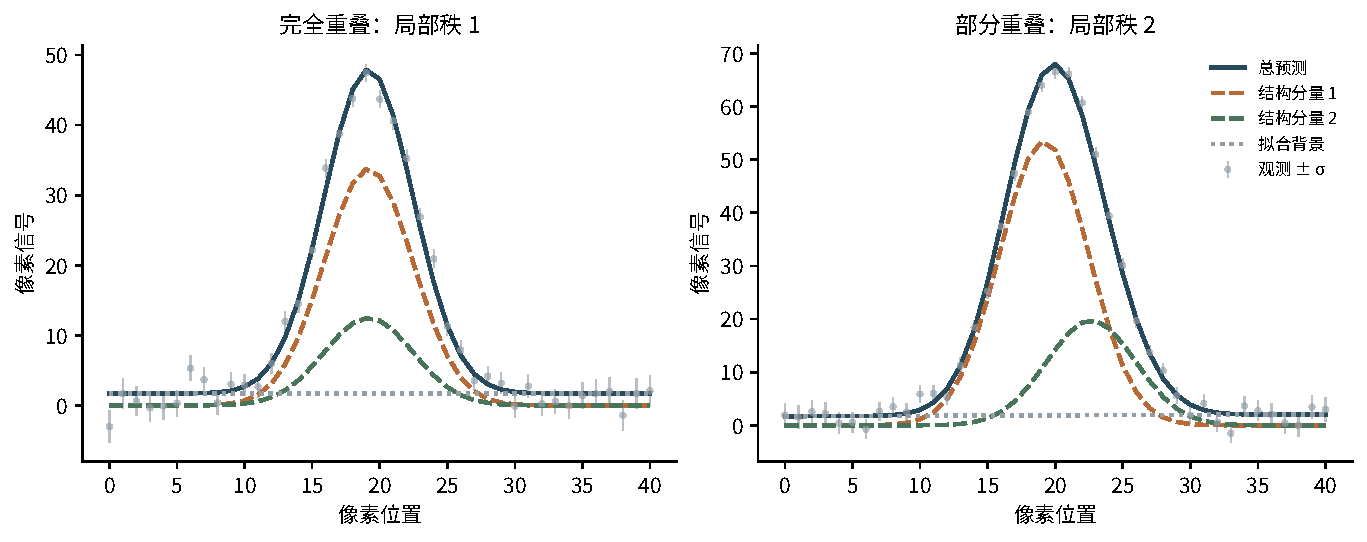
\includegraphics[width=\textwidth]{figures/08_joint_pixels.pdf}
\caption{联合精修的两个合成区域。观测像素只与总预测比较；彩色分量曲线是共享结构给出的解释，并非独立测量。一个区域完全重叠，另一个部分重叠。绘图数据来自本次 7,011 像素的含噪声精修结果。}
\end{figure}

\section{一个必须失败的反例}
若两个晶畴仅互为反演，且没有反常散射，实电子密度满足 $F_{-h}=F_h^*$。于是
\begin{equation}
 \alpha|F_h|^2+(1-\alpha)|F_{-h}|^2=|F_h|^2,
 \qquad\frac{\partial\mu_h}{\partial\alpha}=0.
\end{equation}
任何精修算法都无法从这些数据确定 $\alpha$。优化器可能在平坦方向停在某个值，甚至靠近 0 或 1，但这个值没有测量意义。新接口分别保存内部数值代表和可报告的参数估计；上述情形中比例估计为 \code{null}，并给出秩不足的方向。

这也是闭环的关键约束：结构知识可以缩小一类解释，不能凭空补出实验从未区分过的信息。若必须借助化学先验确定某一方向，应报告先验条件下的结果及其敏感性。

\section{强、弱与复杂孪晶的统一路线}
几何隔离清楚的反射适合提供相位初始化。全部有效区域随后进入共同结构似然，包含弱峰和严重重叠区域。前者负责“找到一个合理起点”，后者负责“检验并改进这个起点”。一批数据在初始化和最后精修中都被使用并不自动造成重复计数；只要最终目标中每份观测只出现一次，初值本身不是第二份测量。

如果没有足够的隔离反射，原生从头求解应明确停止这一分支，要求已有结构假设或其他可验证的相位来源。对混合相、调制结构、显著漫散射或需要动力学散射的情况，也不能继续套用同相运动学模型。

纯计数像素目前由联合泊松信号--背景模块处理，并能对给定结构强度剖面背景。自动的压缩观测求解与 \code{joint-refine} 使用固定方差高斯路径；完整的泊松像素结构优化、几何和吸收联合精修属于下一阶段工程，不能用高斯压缩接口偷偷代替。
